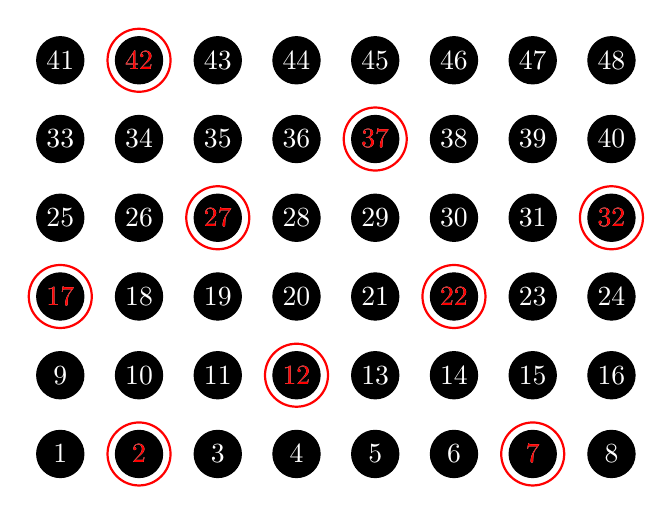
\begin{tikzpicture}
    \foreach \num in {1,2,...,48} {
        \draw[fill=black] ({\num - 8*floor((\num-1) / 8)},{floor((\num-1) / 8)}) circle (0.3) node[white] {\num};
    }
    \foreach \num in {2,7,...,42} {
         \draw[draw=red,thick] ({\num - 8*floor((\num-1) / 8)},{floor((\num-1) / 8)}) circle (0.4) node[red] {\num};
    }
\end{tikzpicture}